\section{Tests of additional meta-parameters}
\lb{sec:app}

In this appendix we discuss tests of some hyper-parameters, which had a relatively little effect on the 
accuracy of the algorithms. For these tests we use the 2-class classification in the 3FGL catalog.

LR algorithm has two hyper-parameters: regularization and tolerance. 
%These features are the limit up to which one wants to go before accepting a solution. 
The effect of the choice of these parameters on accuracy is less than 1\% (Figure \ref{fig:LR_tol_reg}). 
Therefore we used the default values for these parameters (tolerance is 1$e^{-4}$ and regularization parameter is set at 1). The same was used in the 3-class case where the change from GLON to cos(GLON) was seen as the main improvement for LR algorithm.
%\dima{Did we change the regularization in the oversampling 3-class case? I guess it was probably not as important as the change from GLON to cos(GLON).}. 
\begin{figure}[h]
%\centerin
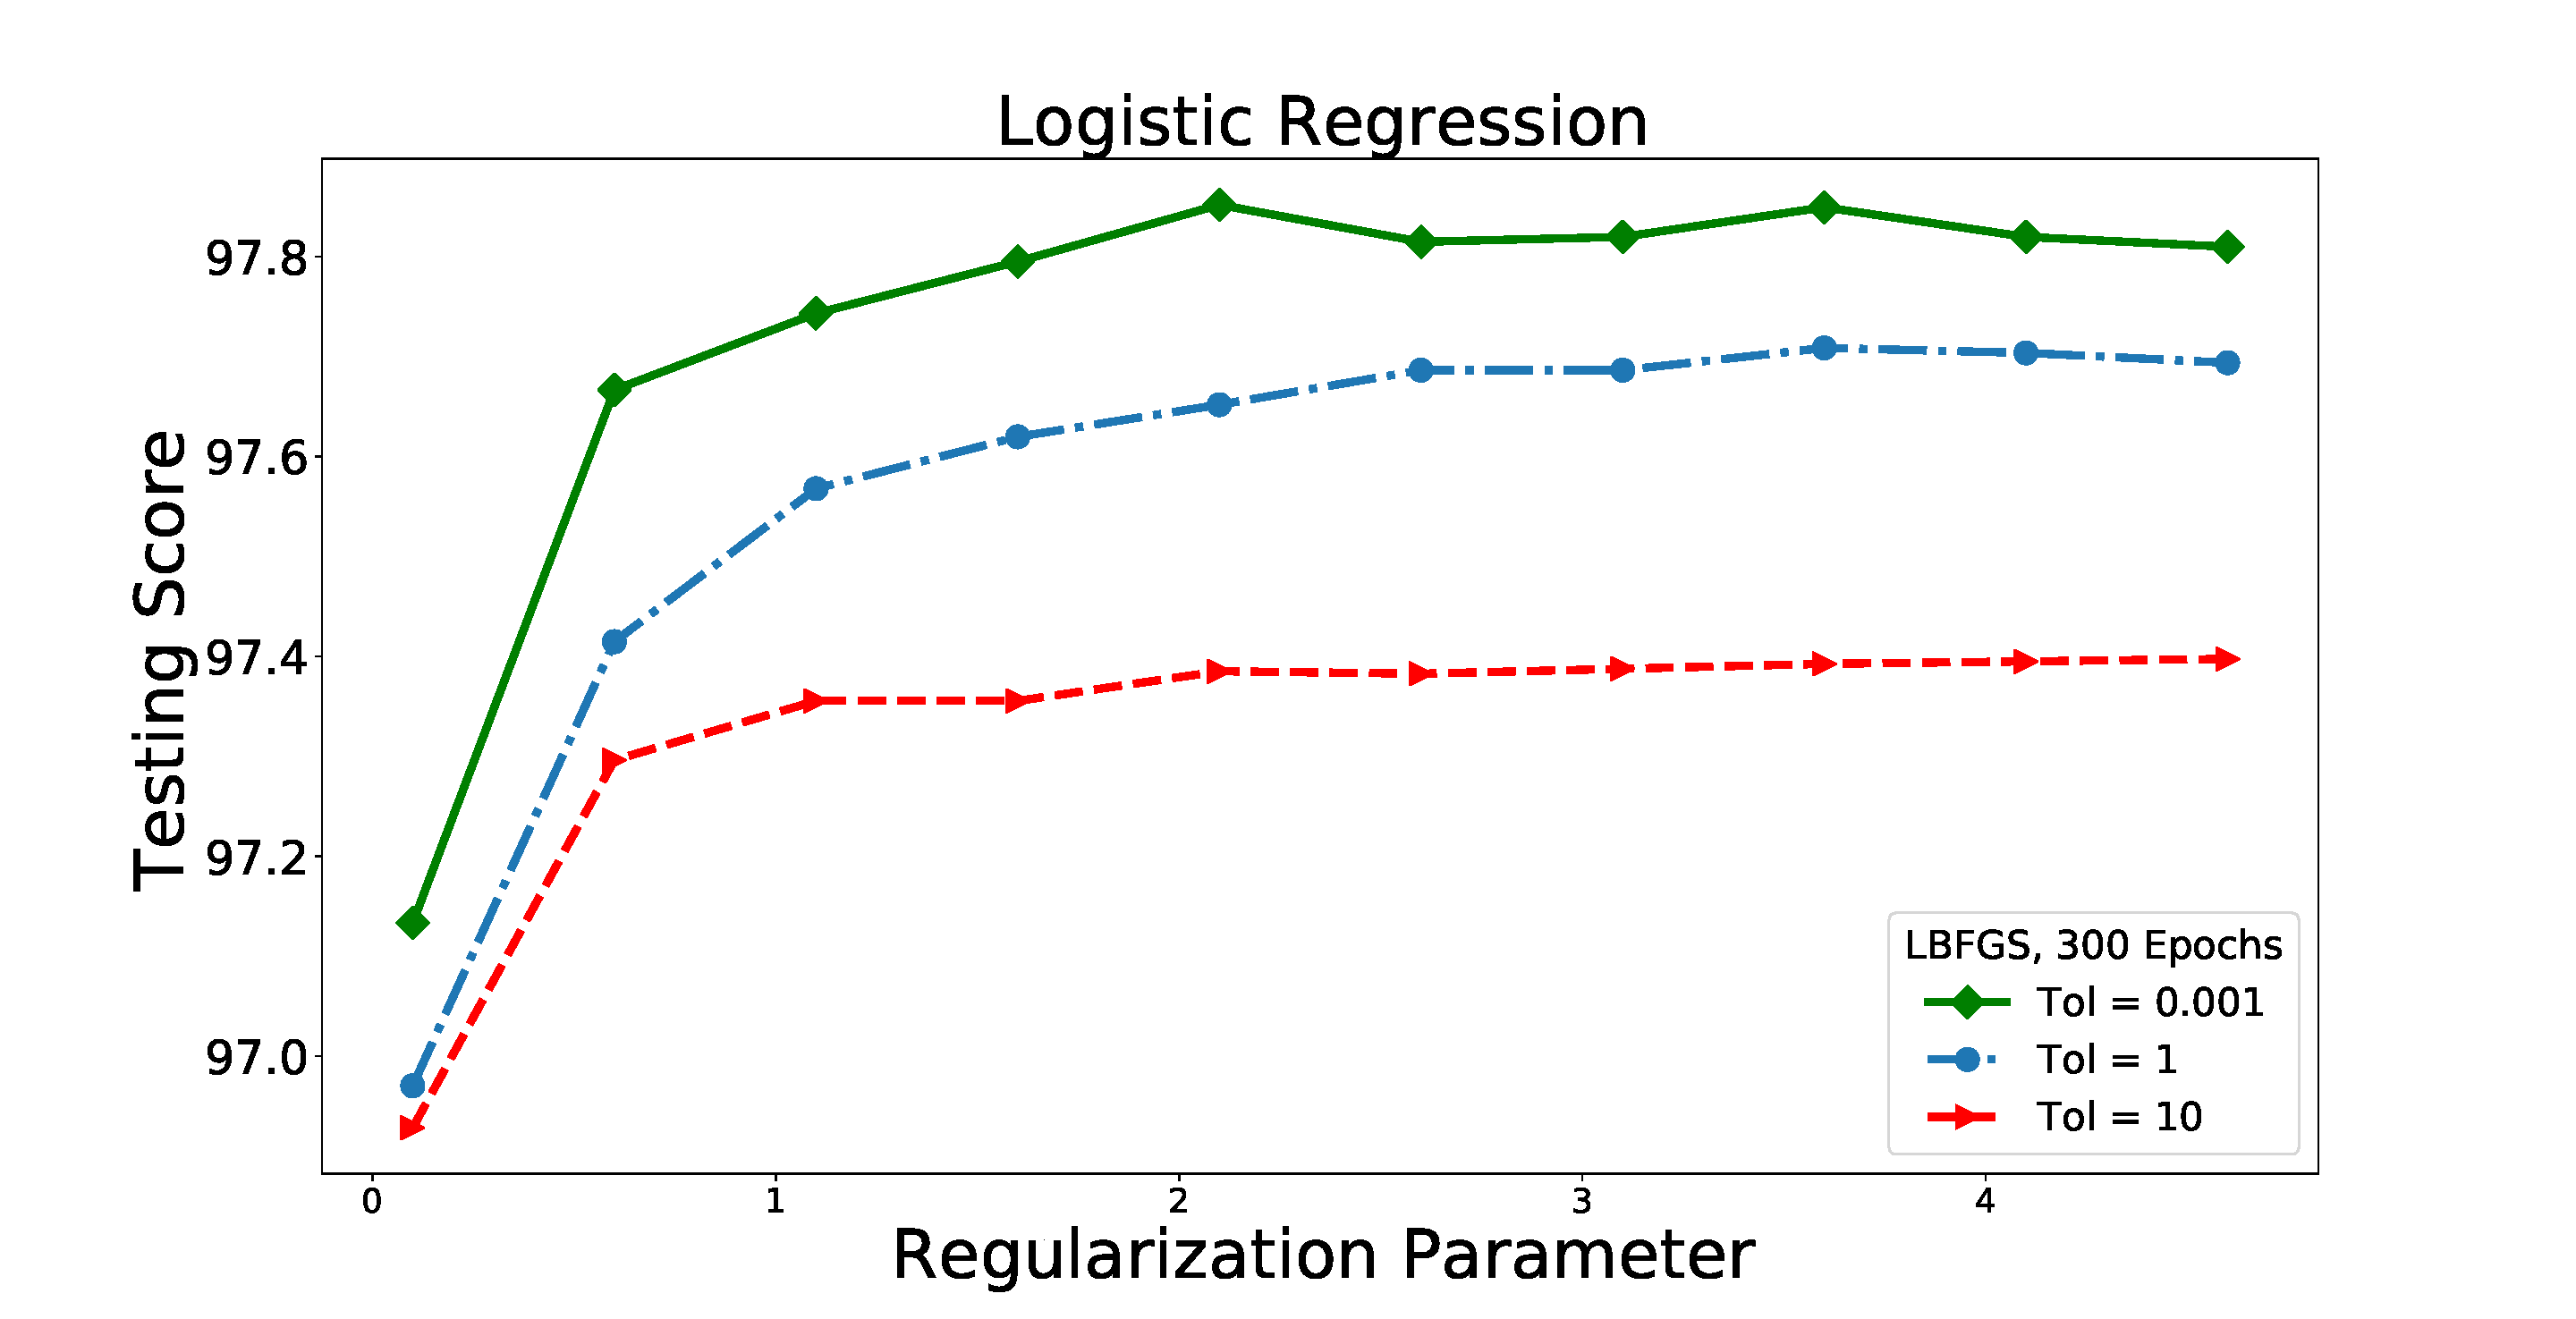
\includegraphics[width=\twopicsp\textwidth]{plots/lr_train_reg.pdf}
%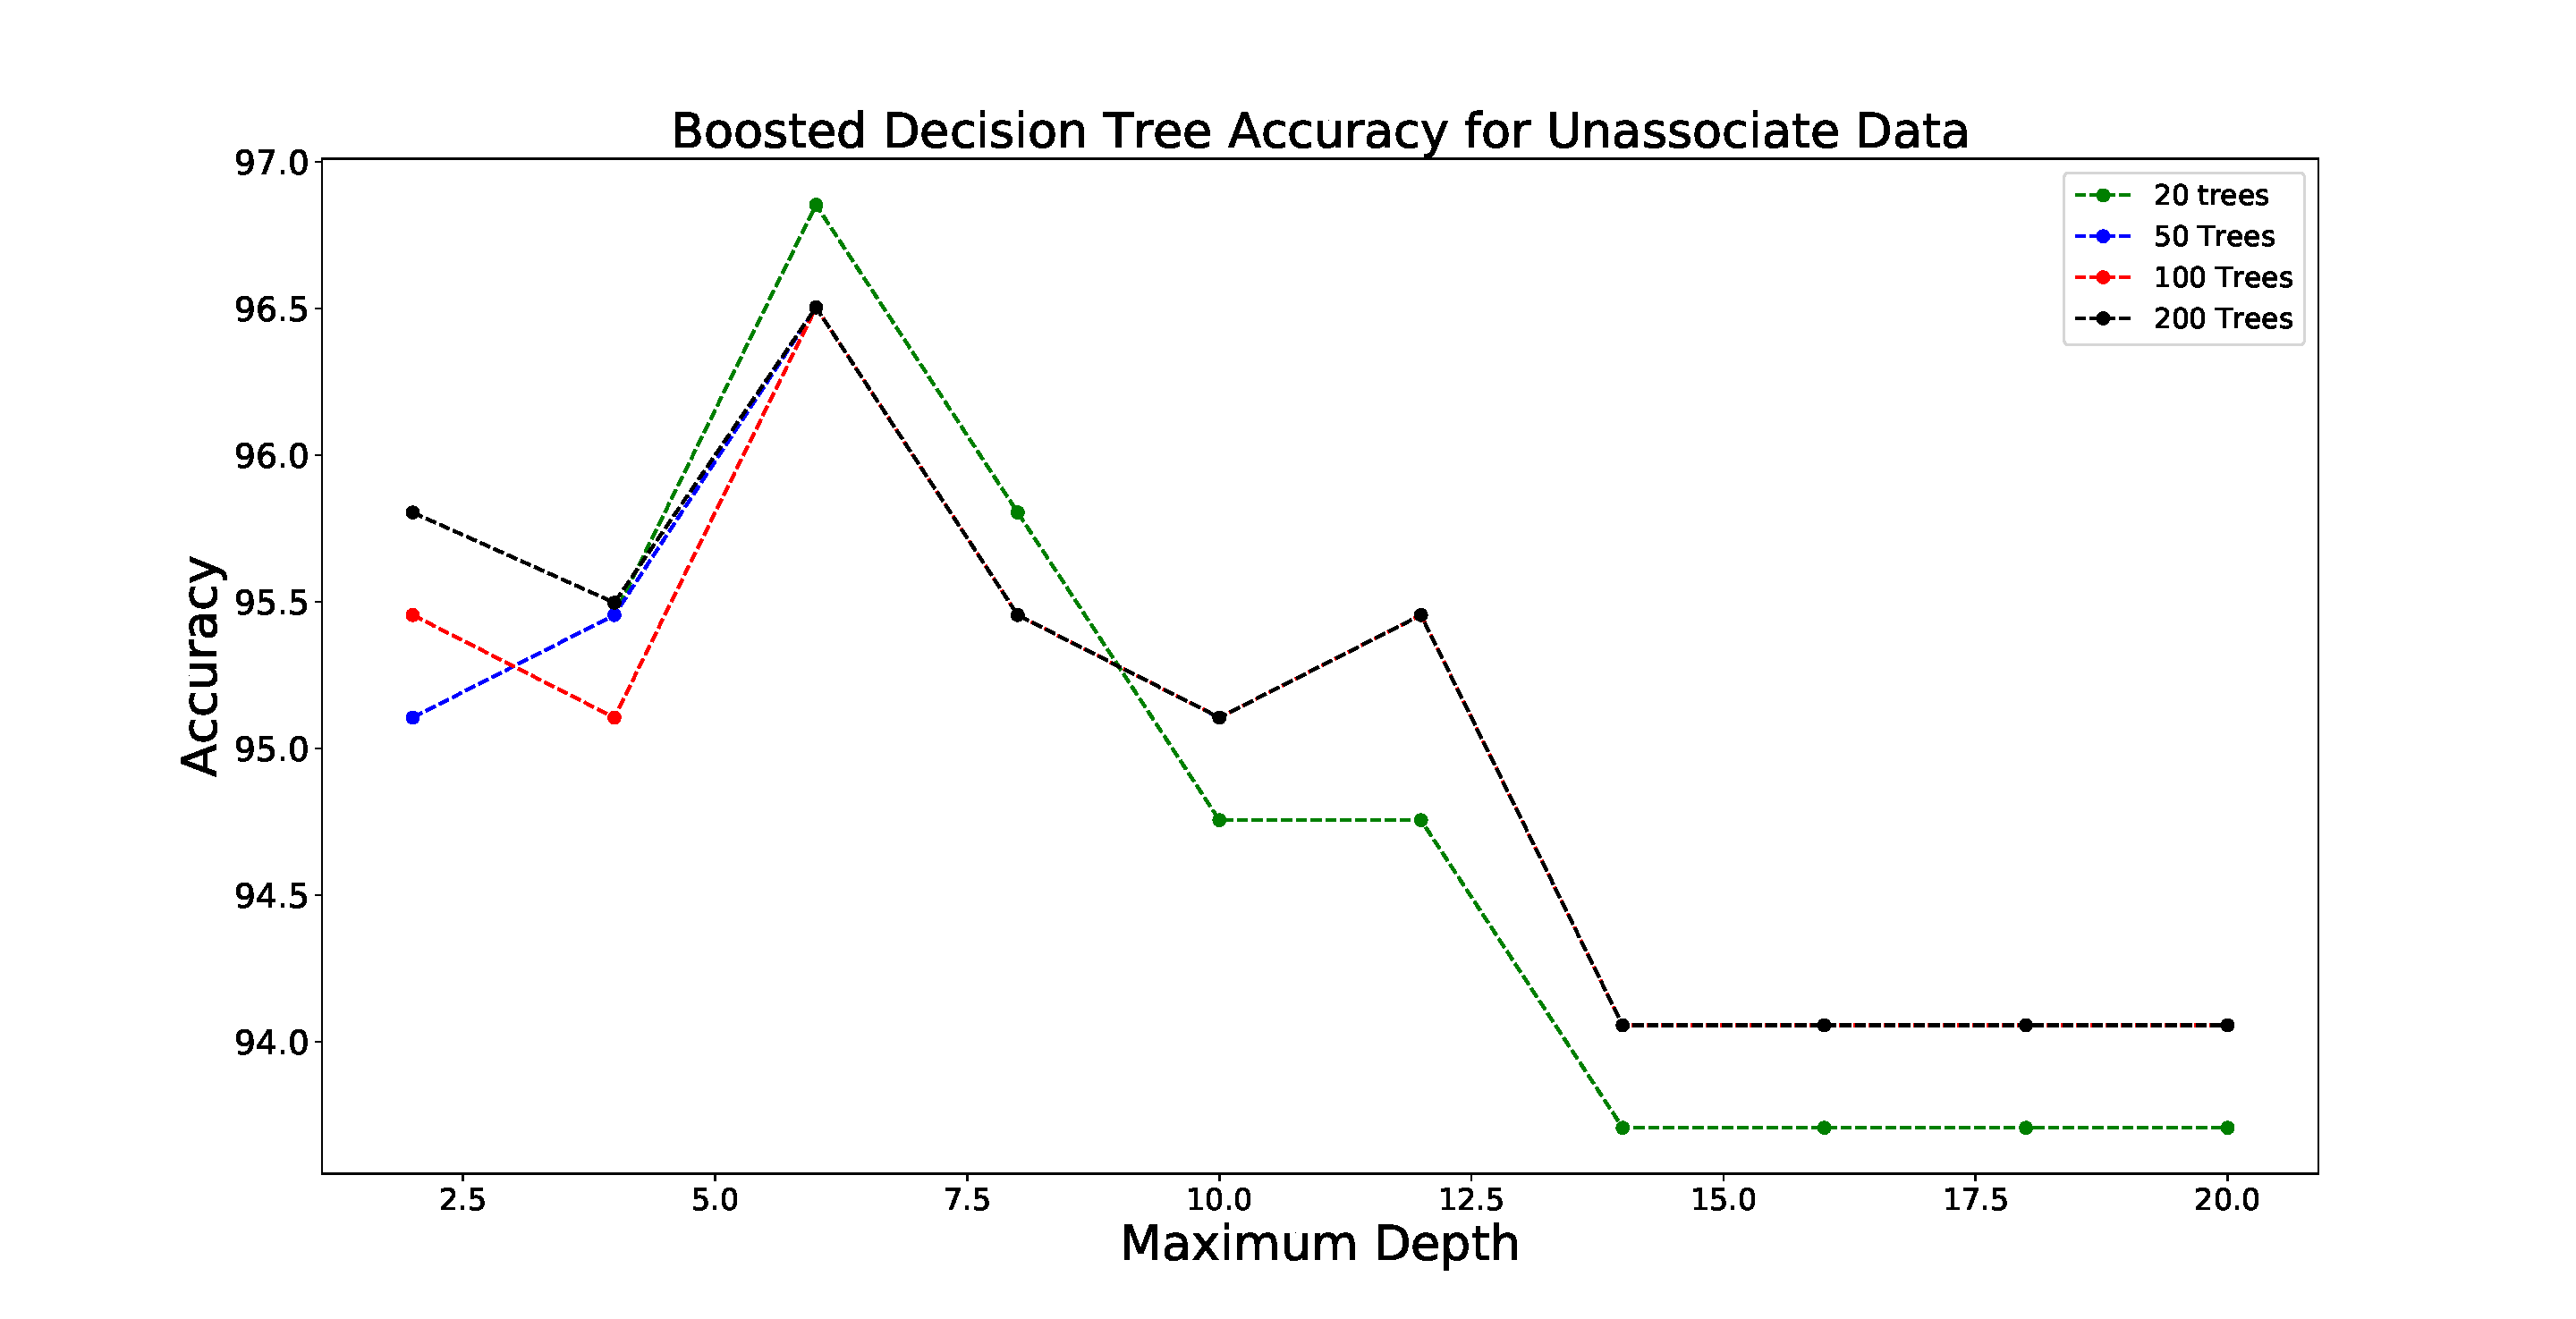
\includegraphics[width=\twopicsp\textwidth]{plots/unassoc_complex.pdf}
\caption{Dependence of LR on tolerance and regularization}
\label{fig:LR_tol_reg}
\end{figure}

In Figure \ref{fig:nn_nn} we show the effect of adding the second hidden layer in the NN algorithm.
The difference between the best accuracies with the additional hidden layer is less then 1\%
compared with the NN with one hidden layer (cf. Table \ref{tab:selected_algs}).
\begin{figure}[h]
%\centerin
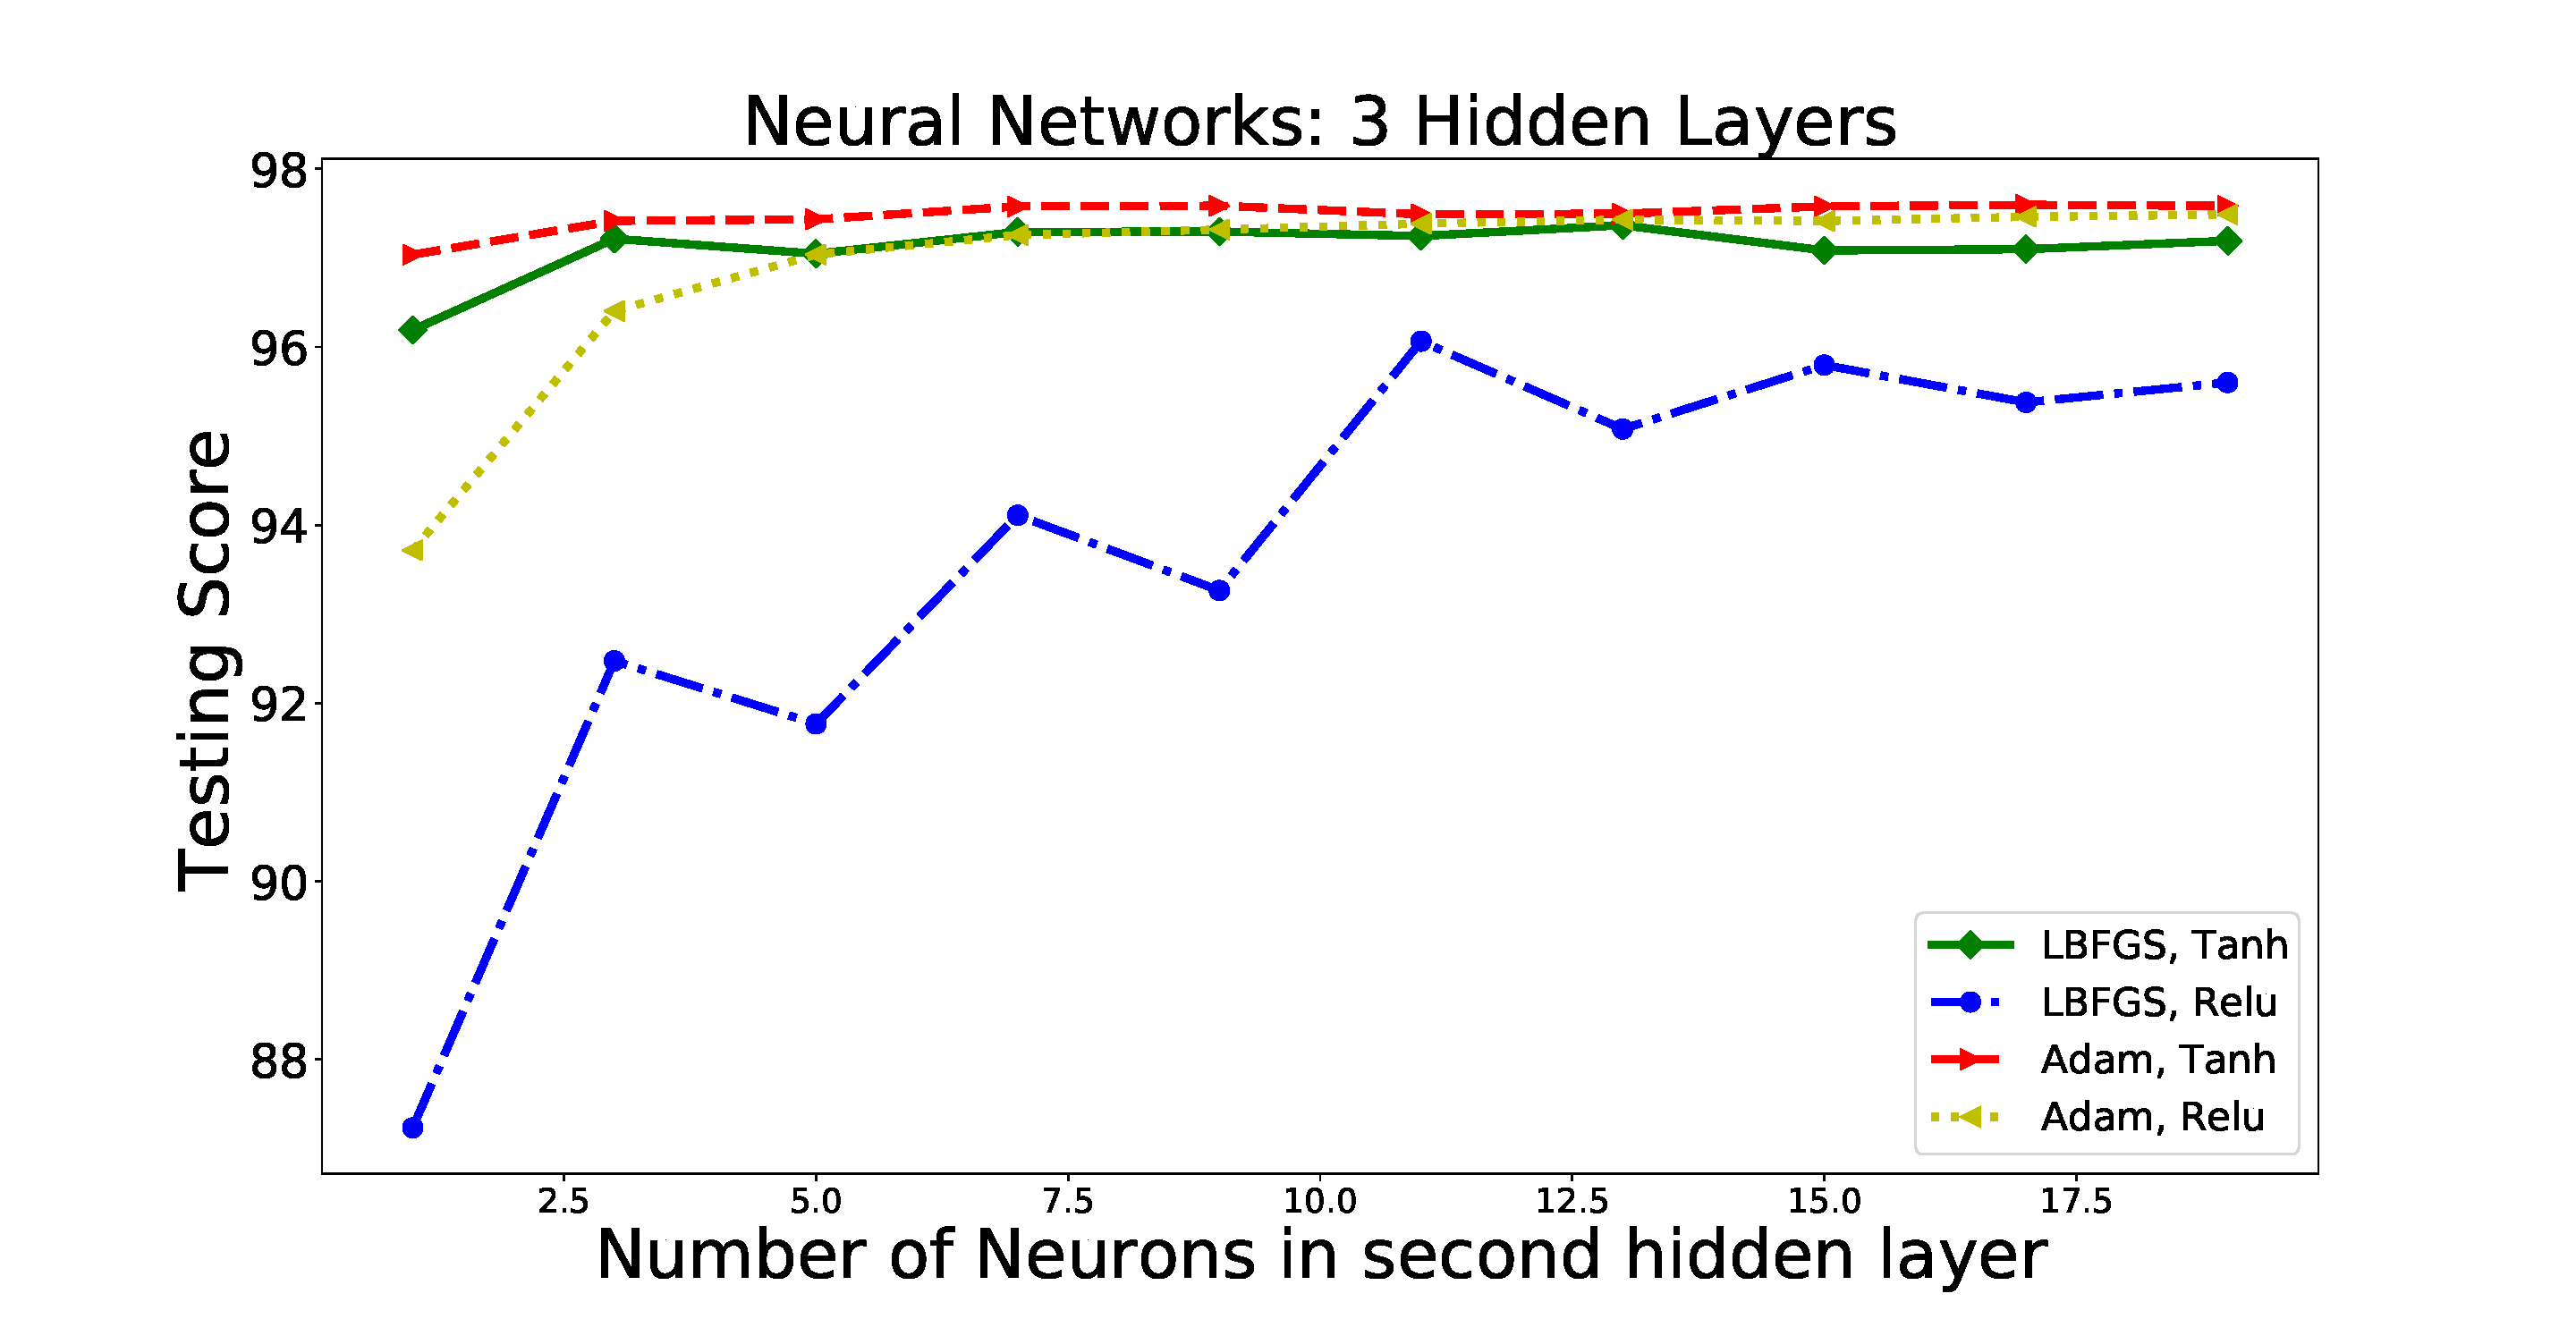
\includegraphics[width=\twopicsp\textwidth]{plots/nn_2layers_3fgl.pdf}
%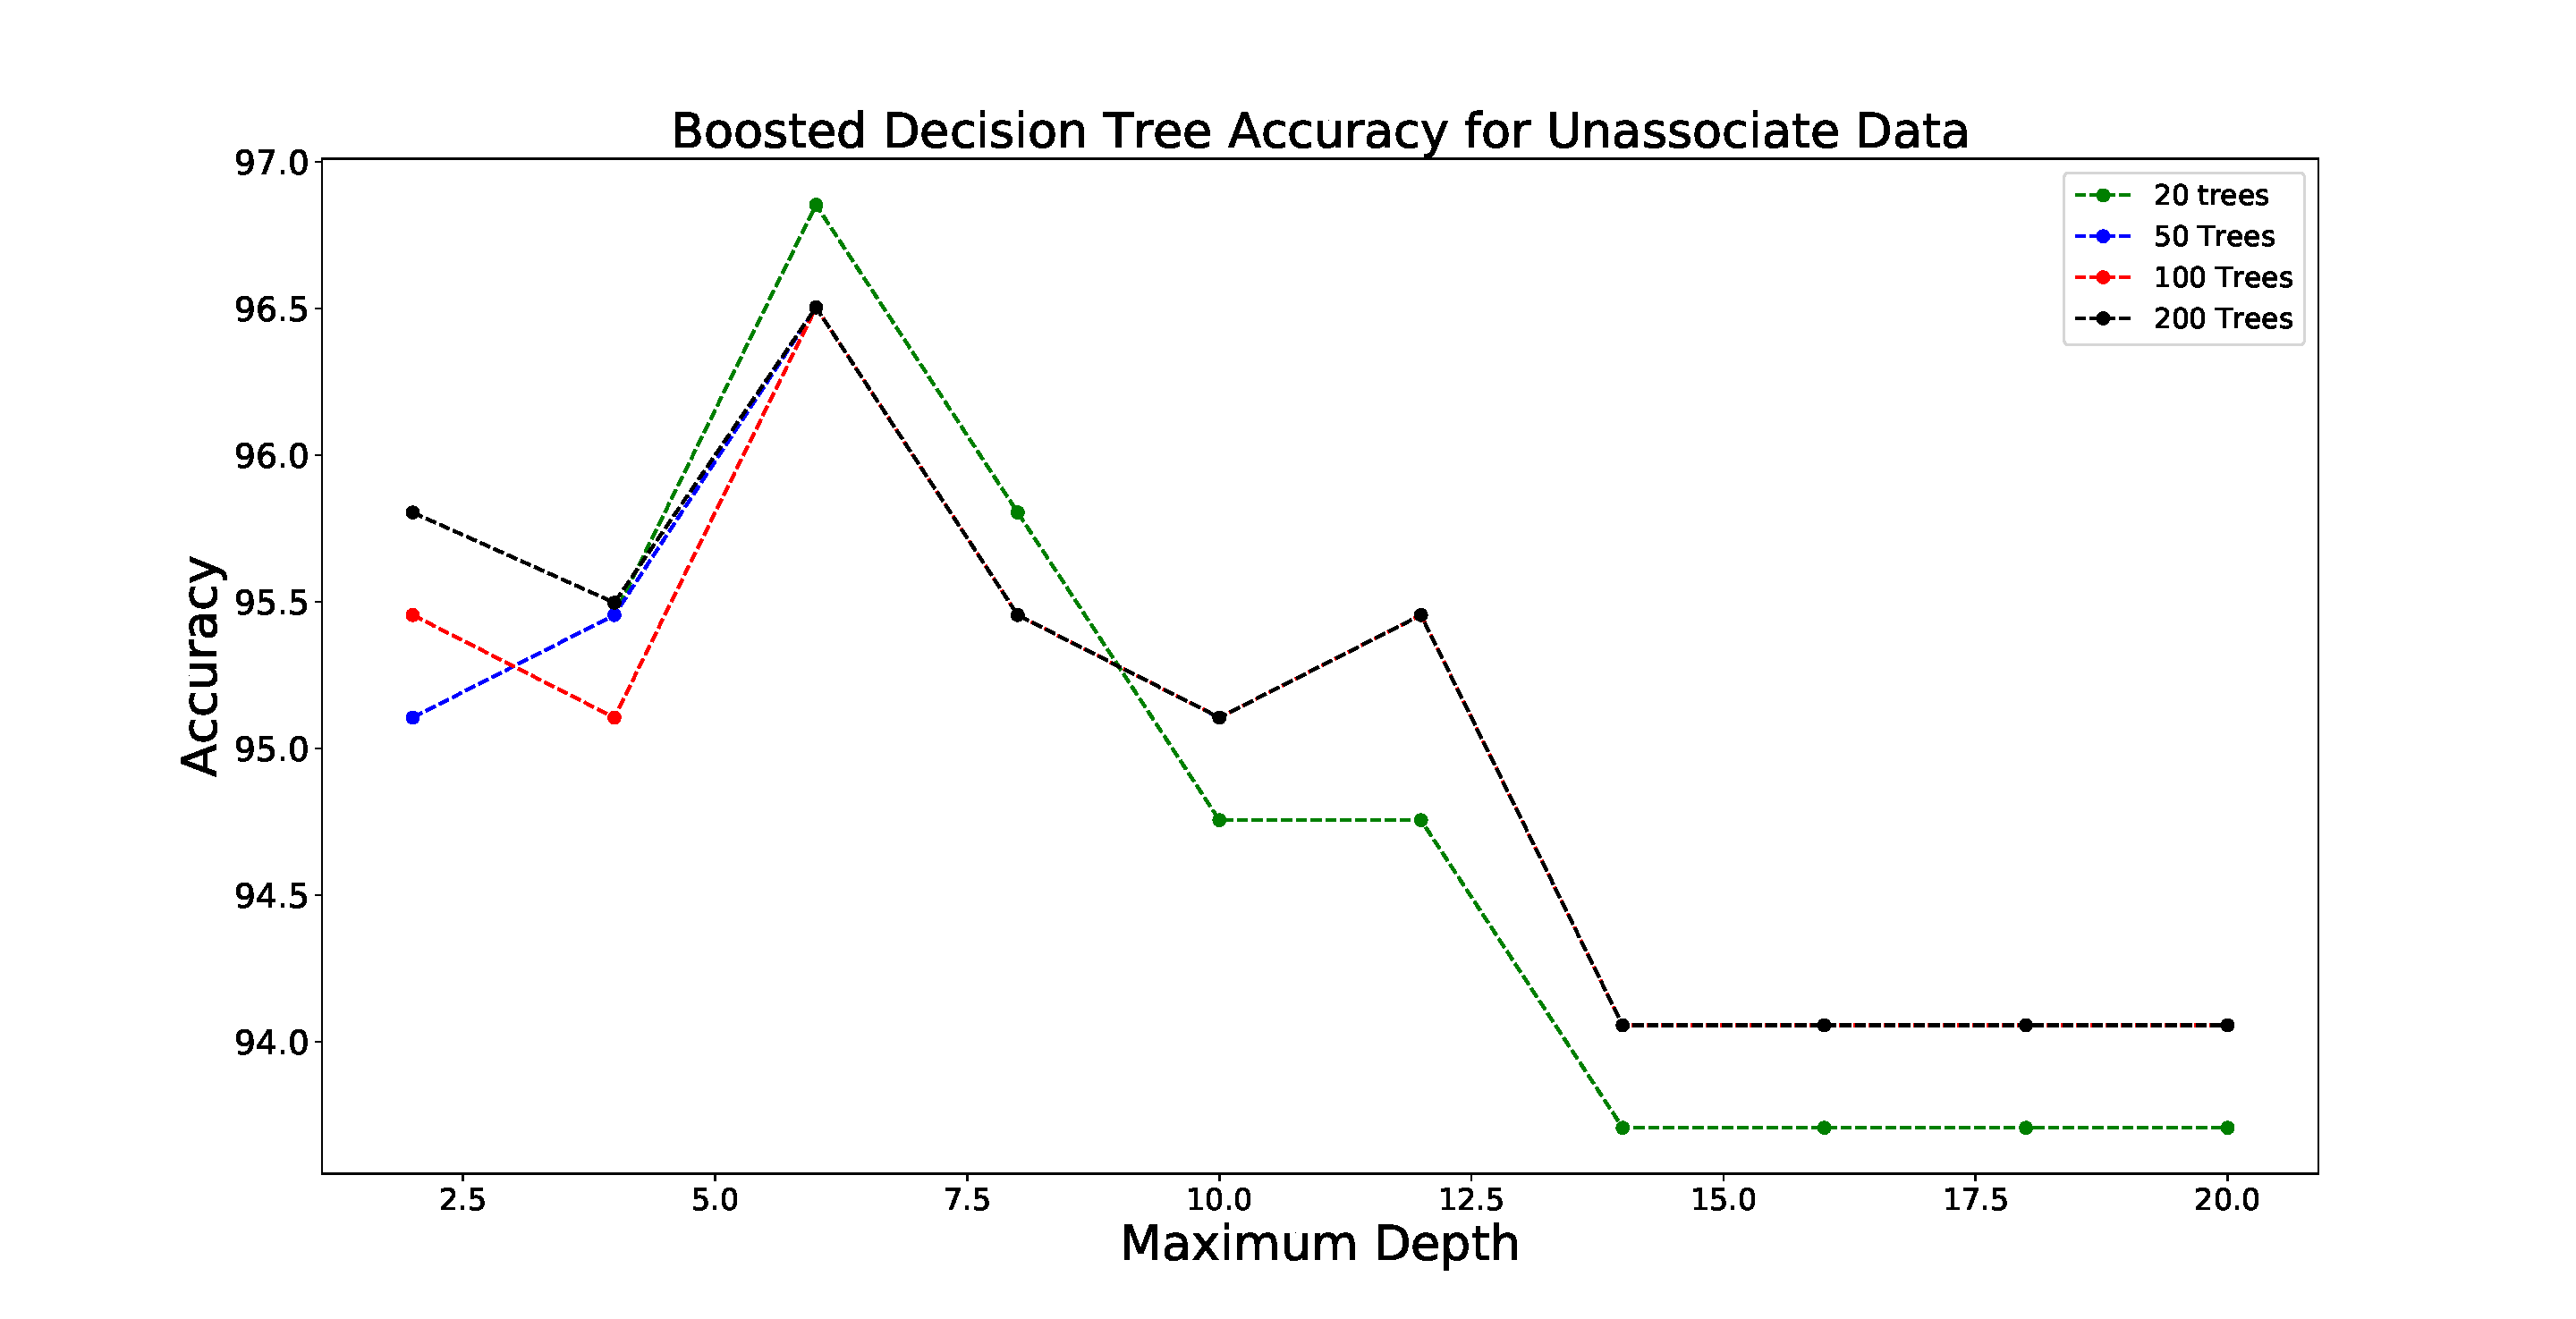
\includegraphics[width=\twopicsp\textwidth]{plots/unassoc_complex.pdf}
\caption{Dependence of NN on the number of neurons in the second hidden layer, for 11 neurons in the first hidden layer.}
\label{fig:nn_nn}
\end{figure}

At the end we summarize features and their statistics,
which we use for probabilistic classification of sources in the 3FGL and 4FGL-DR2 catalogs,
in Tables \ref{tab:3FGL_features} and \ref{tab:4FGL_features} respectively. 

\pgfplotstableread[col sep=comma]{tables/features/3fglassocfeaturesAGNPSRnewfeats.csv}\tablea
\begin{table}
\resizebox{0.45\textwidth}{!}{
\pgfplotstabletypeset[
columns={Name,Mean,SD,Minimum,Maximum},
column type=c,
string type,
every head row/.style={before row=\toprule,after row=\midrule,},
every last row/.append style={after row={\hline} },
every first column/.style={column type/.add={|}{}},
every last column/.style={column type/.add={}{|}},
columns/Name/.style={column name=Feature Name,string replace*={_}{\textunderscore}},
columns/Mean/.style={column name=Mean,column type=c,numeric type,fixed,precision=2},
columns/SD/.style={column name=Standard Deviation,numeric type,fixed,precision=2},
columns/Minimum/.style={column name=Minimum,numeric type,fixed,precision=2},
columns/Maximum/.style={column name=Maximum,numeric type,fixed,precision=2},
skip rows between index={11}{25}
]{\tablea}
}
\vspace{0.2cm}
\caption{Statistics of features used for 2 class probabilistic classification of the 3FGL sources.
\lb{tab:3FGL_features}}
\end{table}

\pgfplotstableread[col sep=comma]{tables/features/4fgldr2agnpsrfeatures.csv}\tableaf
\begin{table}
\resizebox{0.45\textwidth}{!}{
\pgfplotstabletypeset[
columns={Name,Mean,SD,Minimum,Maximum},
column type=c,
string type,
every head row/.style={before row=\toprule,after row=\midrule,},
every last row/.append style={after row={\hline} },
every first column/.style={column type/.add={|}{}},
every last column/.style={column type/.add={}{|}},
columns/Name/.style={column name=Feature Name,string replace*={_}{\textunderscore}},
columns/Mean/.style={column name=Mean,column type=c,numeric type,fixed,precision=2},
columns/SD/.style={column name=Standard Deviation,numeric type,fixed,precision=2},
columns/Minimum/.style={column name=Minimum,numeric type,fixed,precision=2},
columns/Maximum/.style={column name=Maximum,numeric type,fixed,precision=2},
%skip rows between index={17}{28}
]{\tableaf}
}
\vspace{0.2cm}
\caption{Statistics of features used for 2 class probabilistic classification of the 4FGL-DR2 sources.
\lb{tab:4FGL_features}}
\end{table}


